
\documentclass[12pt,a4paper]{scrartcl}

\usepackage[a4paper, left=2cm, right=1cm, bottom=1cm, top=1cm, includeheadfoot]{geometry}
\usepackage[ngerman]{babel}
\usepackage[utf8]{inputenc} % comment this if you uncomment utf8x
%\usepackage[utf8x]{inputenc} % uncomment this if there are problems with 'ä', 'ü', 'ö'
\usepackage{ucs}
\usepackage[usenames,dvipsnames]{xcolor}
\usepackage[fleqn]{amsmath}
\usepackage{amsfonts}
\usepackage{amssymb}
\usepackage{color}
\usepackage{listings}
\usepackage{hyperref}
\usepackage{amsfonts}
\usepackage{pdfpages}
\usepackage{listings}
\usepackage{scrpage2}
\usepackage{graphicx}


\definecolor{mygray}{rgb}{0.9,0.9,0.9}
\lstset{language=[Visual]Basic, morekeywords={param, local}}


\lstset{
   literate={ö}{{\"o}}1
           {ä}{{\"a}}1
           {ü}{{\"u}}1
           {ß}{{\ss}}1
           {é}{{\'e}}1,
   inputencoding=ansinew,
   extendedchars=true,
   basicstyle=\scriptsize\ttfamily,
   numberstyle=\scriptsize,
   breaklines=true,
   tabsize=2,
   numbersep=5pt
}
\lstdefinestyle{customcpp}{
   language=C++,
   backgroundcolor=\color{mygray},
   numbers=left,
   keywordstyle=\color{blue}\bfseries,
   stringstyle=\color{BrickRed}\ttfamily,
   commentstyle=\color{OliveGreen}\ttfamily,
   showspaces=false,
   showstringspaces=false,
   showtabs=false
}
\lstdefinestyle{customoutput}{
   backgroundcolor=\color{mygray},
   numbers=none,
   showspaces=false,
   showtabs=false
}

\newcommand{\sourceCode}[1]{\lstinputlisting[style=customcpp]{#1}}
\newcommand\tab[1][1cm]{\hspace*{#1}}
%****************** self defined commands ***************************
%include a .cpp source file
%usage: \cppfile{../path_to_your_file/filename}
\newcommand{\cppfile}[1]{
\begin{itemize}
\item[]\lstinputlisting[caption="#1.cpp",label="#1.cpp", style=customcpp]{#1.cpp}
\end{itemize}
}

%include a .c source file
%usage: \cfile{../path_to_your_file/filename}
\newcommand{\cfile}[1]{
\begin{itemize}
\item[]\lstinputlisting[caption="#1.c",label="#1.c", style=customcpp]{#1.c}
\end{itemize}
}

%include a code snippet
%usage: \hfile{../path_to_your_file/filename}{startline}{endline}
\newcommand{\csnippet}[3]{
\begin{itemize}
\item[]\lstinputlisting[caption=#1.c, style=customcpp, firstline=#2,lastline=#3]{#1.c}
\end{itemize}
}

%include a .h source file
%usage: \hfile{../path_to_your_file/filename}
\newcommand{\hfile}[1]{
\begin{itemize}
\item[]\lstinputlisting[caption="#1".h,label="#1.h", style=customcpp]{#1.h}
\end{itemize}
}

%include a module (.cpp and .h)
%usage: \hfile{../path_to_your_file/filename}
\newcommand{\cppmodul}[1]{
\begin{itemize}
\item[]\lstinputlisting[caption=#1.h,label=#1.h, style=customcpp]{#1.h}
\item[]\lstinputlisting[caption=#1.cpp,label=#1.cpp, style=customcpp]{#1.cpp}
\end{itemize}
}

%include a module (.c and .h)
%usage: \hfile{../path_to_your_file/filename}
\newcommand{\cmodul}[1]{
\begin{itemize}
\item[]\lstinputlisting[caption=#1.h,label=#1.h, style=customcpp]{#1.h}
\item[]\lstinputlisting[caption=#1.c,label=#1.c, style=customcpp]{#1.c}
\end{itemize}
}

%include a code snippet
%usage: \hfile{../path_to_your_file/filename}{startline}{endline}
\newcommand{\snippet}[3]{
\begin{itemize}
\item[]\lstinputlisting[caption=#1.cpp,label=#1.cpp, style=customcpp, firstline=#2,lastline=#3]{#1.cpp}
\end{itemize}
}

%include a test-output file 
%usage: \testoutput{../path_to_your_file/filename}
\newcommand{\testoutput}[1]{
\begin{itemize}
\item[]\lstinputlisting[caption=#1]{#1.txt}
\end{itemize}
}

%include a .s source file
%usage: \assemblerfile{../path_to_your_file/filename}

\newcommand{\assemblerfile}[1]{
\begin{itemize}
\item[]\lstinputlisting[caption=#1.s ,label=#1.s , style=customassembler]{#1.s}
\end{itemize}
}

%include a code snippet
%usage: \hfile{../path_to_your_file/filename}{startline}{endline}
\newcommand{\assemblersnippet}[3]{
\begin{itemize}
\item[]\lstinputlisting[caption=#1.s, style=customassembler, firstline=#2,lastline=#3]{#1.s}
\end{itemize}
}


 %beinhaltet alle benötigten Packages etc.
\begin{document}

\title{SDP - Uebung 1} % Übungsname und Nummer angeben
\subtitle{Wintersemester 2019/20} % Semester angeben oder auskommentieren, falls nicht erwünscht
\author{Adam Kensy - S1810306018\\
		Philipp Holzer - S1810306028} % Autorenname
\date{\today}
%date{} % Das heutige Datum automatisch einfügen

\maketitle % Titelseite erstellen

\newpage
\tableofcontents % Inhaltsverzeichnis erstellen
\newpage

% Kure Befehlsreferenz
%\section{} erstellt eine Überschrift
%während
%\subsection{} eine Unterüberschrift erstellt
% Eine neue Seite wird mit \newpage erstellt

\section{Organisatorisches}

\subsection{Team}
\begin{itemize}
	\item Philipp Holzer, Matr.-Nr.: 1810306028
	\item Adam Kensy, Matr.-Nr.: 1810306018
\end{itemize}

\subsection{Aufteilung und Verantwortlichkeitsbereiche}
\begin{itemize}
	\item Philipp Holzer
		\begin{itemize}
		\item Planung
		\item Klassendiagramm
		\item Implementierung und Testen der Klassen
			\begin{itemize}
			\item Logbook
			\item Vehicle
			\end{itemize}
		\item Dokumentation
		\end{itemize}
	\item Adam Kensy
		\begin{itemize}
		\item Planung
		\item Klassendiagramm
		\item Implementierung und Testen der Klassen
			\begin{itemize}
			\item Carpool
			\item Vehicle
			\item Car, Truck, Motorcycle
			\end{itemize}
		\item Dokumentation
		\end{itemize}
\end{itemize}

\subsection{Aufwand}
\begin{itemize}
	\item Philipp Holzer		\tab geschätzt: 7	\tab tatsächlich: 8
	\item Adam Kensy		\tab  geschätzt:	7	\tab  tatsächlich: 5
\end{itemize}

% Für eine numerierte Aufzählung verwendet man 

%\begin{enumerate}
%	\item 
%\end{enumerate}

%%%%%%%%%%%%%%%%%%%%%%%%%%%%%%%
\newpage
\section{Anforderungsdefinition (Systemspezifikation)}

Gesucht ist ein Fuhrpark wo man verschiedene Fahrzeuge verwalten kann. Die Fahrzeuge besitzen jeweils ein Kennzeichen, Marke und ein Fahrtenbuch.
Der Fuhrpark hat keine Begrenzung bei der Menge an Fahrzeugen, jedoch kann jedes Kennzeichen nur einmal vorkommen. 


%%%%%%%%%%%%%%%%%%%%%%%%%%%%%%%
\section{Systementwurf}

\subsection{Klassendiagramm}
 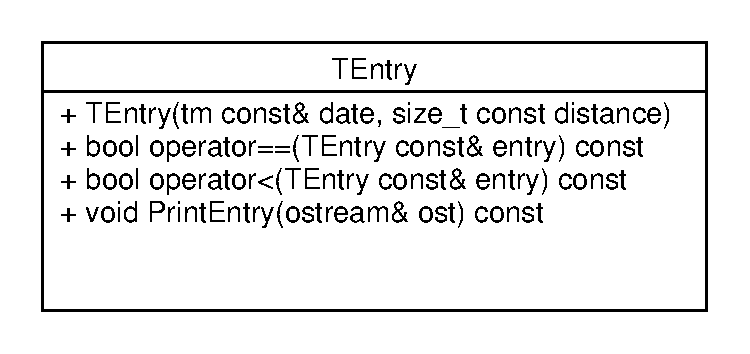
\includegraphics[scale = 0.40]{UML-Diagram.pdf}

\subsection{Klassendiagramm durch Visual Studio}
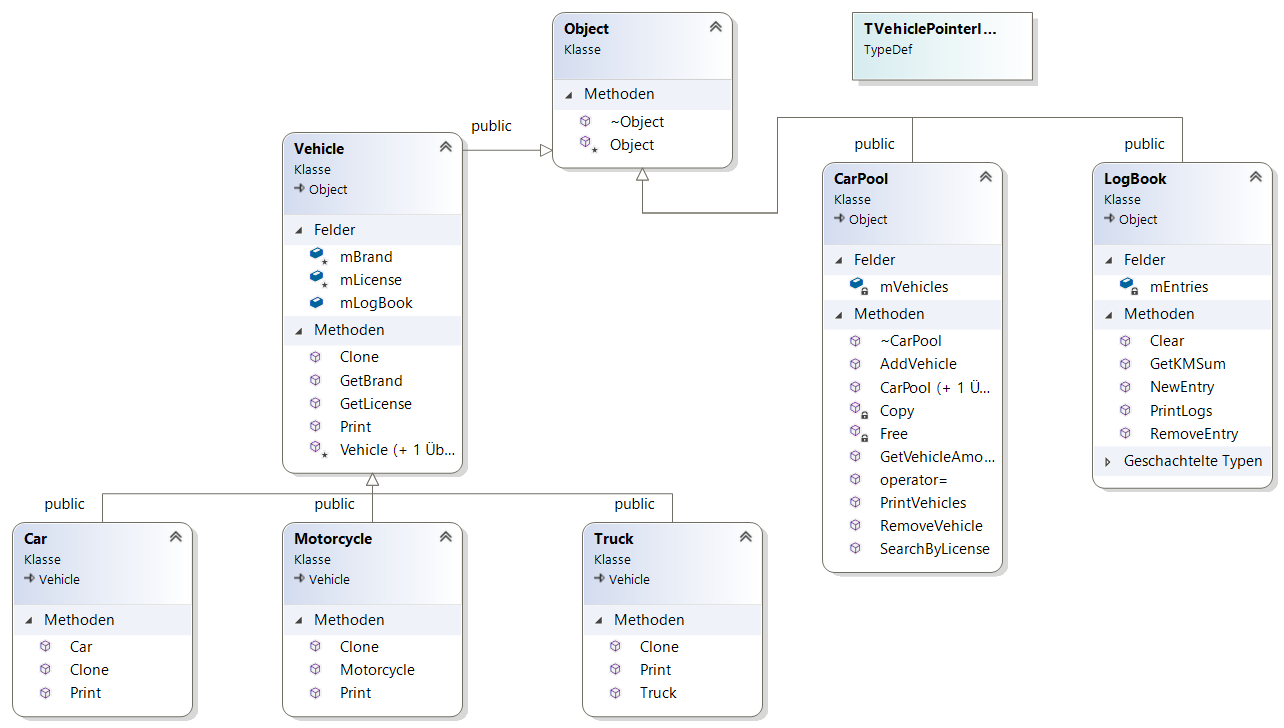
\includegraphics[scale=0.65]{./CarPool/ClassDiagram.png}

%%%%%%%%%%%%%%%%%%%%%%%%%%%%%%%
\subsection{Komponentenübersicht}

\begin{itemize}

\item \textbf{Klasse \string"Object"} \\
Basis aller Klassen

\item \textbf{Klasse "Carpool"}
\\ Verwaltet alle Fahrzeuge
\\ Besitzt eine Ausgabefunktion um alle enthaltenen Fahrzeuge auszugeben

\item \textbf{Klasse "Logbook"}
\\ Das Fahrtenbuch der Fahrzeuge
\\ Vor der Ausgabe wird das Fahrtenbuch immer nach Datum sortiert

\item \textbf{Klasse "Vehicle"}
\\ Stellt die Fahrzeuge dar, dazu gehören: PKW, LKW, Motorräder

\item \textbf{Klasse "Car", "Truck", "Motorcycle"}
\\ Konkrete Objekte für die Fahrzeuge
\\ Besitzen nur eine Ausgabefunktion, wobei der Ausgabeoperator überschrieben ist

\end{itemize}

\subsection{Designentscheidungen}
\begin{itemize}
\item Es wurde keine EBNF erstellt da es international anwendbar sein soll. 
\item Der Fuhrpark redet mit uns über die Konsole wenn etwas schiefläuft -> wenn kein Fahrzeug hinzugefügt oder entfernt werden konnte bekommen wird eine Fehlermeldung aber ansonsten bleibt der Fuhrpark ruhig. 
\item Wir haben uns entschieden, dass das Einfügen und Entfernen über Pointer läuft - wir dachten uns, es macht so am meisten Sinn denn man parkt das Fahrzeug irgendwo und teilt dies dann der Verwaltung mit. 
\item Dadurch, dass wir mit Pointer arbeiten haben wir beim Carpool die Rule-Of-Three angewandt. 
\item Wir benutzen die tm-Struktur für Datums-Angaben und erwarten uns eine sinnvolle Eingabe vom Anwender. 
\item Es wird sortiert ins Fahrtenbuch eingetragen, dies macht am meisten Sinn, da man dies direkt nach einer Fahrt macht. 
\end{itemize}

%%%%%%%%%%%%%%%%%%%%%%%%%%%%%%%
%\section{Dateibeschreibung}

%Hier werden die verwendeten Dateien beschrieben, sofern Informationen aus externen
%Dateien gelesen bzw. in diese geschrieben werden. Eine solche Beschreibung umfasst...

%%%%%%%%%%%%%%%%%%%%%%%%%%%%%%%


%%%%%%%%%%%%%%%%%%%%%%%%%%%%%%%
%\section{Komponentenentwurf}

%Immer mit subsections die einzelnen Klassen genauer erläuten.

%%%%%%%%%%%%%%%%%%%%%%%%%%%%%%%
\newpage
\section{Testprotokollierung}

%Im Testprotokoll werden die Testdaten und die Testergebnisse für alle Testfälle beschrieben. Weiters muss die Testumgebung angeführt sein (welches %Testframework
%wurde verwendet, mit welchen Komponentenversionen wurde gestestet, welche Stubs
%wurden verwendet, etc). Wenn die Komponenten und Subsysteme getrennt getestet
%wurden, ist die Testprotokollierung für die Komponenten getrennt anzugeben. Weiters sind identifizierte Schwachstellen und Probleme festzuhalten.

\subsection{Testumgebung}

Microsoft Visual Studio Enterprise 2019\\
Version 16.3.5\\
Microsoft Visual C++ 2019\\
\\
Windows 10, 64Bit, Build 18362\\
\\
Testdriver: main.cpp

\subsection{Testausgabe}
\lstinputlisting{test_output.txt}

%%%%%%%%%%%%%%%%%%%%%%%%%%%%%%%
%\section{Tabellen und Diagramme}

%Ergänzende und unterstützende Tabellen und Diagramme können am Ende der Systemdokumentation angefügt werden.

% Zur Info: Tabellen am besten in Excel erstellen und dann als Bild hier einfügen - Tabellen können in Latex sehr unangenehm werden!!
% Befehl um Bilder einzufügen:
%\includegraphics{Relativer/Pfad/zum/Bild.Endung}

%%%%%%%%%%%%%%%%%%%%%%%%%%%%%%%
%\section{Software-Qualitätsmetriken}

%Metriken dienen dazu, die Qualität von Software zu messen. Für C++ gibt es hier
%etwa das frei verfügbare Programm CCCC, welches für Linux und Windows unter
%der Adresse http://sourceforge.net/projects/cccc verfügbar ist. Für einen gegebenen
%Souce Code werden die Metriken ermittelt und ausgegeben. Eine (kompakte und auf
%das Wesentliche gekürzte) Ausgabe kann hier auf freiwilliger Basis aufgenommen
%werden und dient als Referenz bei Wartungsarbeiten (Degeneration des Codes und
%Designs).

%%%%%%%%%%%%%%%%%%%%%%%%%%%%%%%
\section{Quellcode}

\subsection{Object}
\cppmodul{CarPool/Object}

\subsection{CarPool}
\cppmodul{./CarPool/CarPool/CarPool}

\subsection{Vehicles}
\cppmodul{./CarPool/Vehicles/Vehicle}
\cppmodul{./CarPool/Vehicles/Car}
\cppmodul{./CarPool/Vehicles/Truck}
\cppmodul{./CarPool/Vehicles/Motorcycle}

\subsection{LogBook}
\cppmodul{./CarPool/LogBook/LogBook}

\subsection{main}
\cppfile{./CarPool/main}

% Um Quellcode einzufügen einfach diesen Befehl verwenden:
%\sourceCode{Relativer/Pfad/zum/SourceCode.Endung}

\end{document}